\documentclass[12pt, a4paper]{article}
\title{\textbf{Laser Pointer Based Human-Computer-Interaction using Computer-Vision}}

\usepackage[labelformat=empty]{caption}
\usepackage{graphicx}
\usepackage{wrapfig}
\usepackage{listings}
\usepackage[hidelinks=true]{hyperref}
\usepackage{mathtools}
\usepackage{pgfgantt}
\usepackage{tocloft}
\usepackage{tocbibind}
\usepackage{indentfirst}
\usepackage{mathtools}
\usepackage{acronym}
\usepackage[acronym]{glossaries}

\makeglossaries
\begin{document}
\pagenumbering{roman}
\subsection*{COPYRIGHT}
	\vspace{0.5cm}

The author has agreed that the Library, Department of Electronics and Computer Engineering, Pulchowk Campus, Institute of Engineering may make this report freely available for inspection. Moreover, the author has agreed that permission for extensive copying of this project report for scholarly purpose may be granted by the supervisors who supervised the project work recorded herein or, in their absence, by the Head of the Department wherein the project report was done. It is understood that the recognition will be given to the author of this report and to the Department of Electronics and Computer Engineering, Pulchowk Campus, Institute of Engineering in any use of the material of this project report. Copying or publication or the other use of this report for financial gain without approval of to the Department of Electronics and Computer Engineering, Pulchowk Campus, Institute of Engineering and author’s written permission is prohibited.

Request for permission to copy or to make any other use of the material in this report in whole or in part should be addressed to:

\vspace{0.2cm}
\begin{flushleft}

Dibakar Raj Pant, PhD\\
Head of Department\\
Department of Electronics \& Computer Engineering\\
Pulchowk Campus, Institute of Engineering\\
Pulchowk, Lalitpur\\
Nepal
\end{flushleft}


\addcontentsline{toc}{subsection}{Copyright}

\newpage
\subsection*{ACKNOWLEDGEMENT}
		\vspace{0.5cm}	

We would like to express our deep sense of gratitude to our project supervisor, Dr. Dibakar Raj Pant, Head of Department, Department of Electronics and Computer Engineering, Pulchowk Campus, for providing us with a lot of inspiration and intellectual guidance while being very encouraging and supportive.

We are highly indebted to the Department of Electronics and Computer Engineering, Pulchowk Campus for providing us with this opportunity of collaborative undertaking which has helped us develop a major project of our own that greatly enhances our knowledge and provides a new experience of team-work, quite important for our future career.

We would also like to thank the Village Tech Solutions for believing in us and providing us the opportunity to work on this project.

We would like to express our sincere gratitude to the Robotics Club, Pulchowk Campus and its members for providing us the various machineries and tools required to complete the hardware of the project.

Last but not the least, we would like to thank everyone who provided us with guidance and support during the project.

\addcontentsline{toc}{subsection}{Acknowledgement}

\newpage
\subsection*{ABSTRACT}
	\vspace{0.5cm}	
        With the advancement in field of technology, various techniques have been developed with the aim of improving the interactivity in the education system. As classrooms may contain a large number of students each from diverse environment, an effective interaction tool is a necessity these days. The same situation may also arise in the conferences. Video projection is in widespread use for multimedia presentations in classrooms and in conferences. 

A particular application is the interactive demonstration of software with a computer whose screen content is sent to a video beamer. An uncomfortable aspect here is that the usual keyboard/mouse computer limits the possibilities of the speakers by tying them to the location of the computer with its devices of interaction. To avoid this restriction, we have developed a system using a common laser pointer tracked by a video camera as an input device. Video cameras already present in multimedia lecture rooms can be used for this purpose, which reduces the required overhead compared to special tracking devices, like electro-magnetic ones. Compared to video-based gesture recognition or tracking of a pointing stick, video-tracking of a laser point is less sensitive to variations in the ambient
light.

The project is, technically, divided into two parts – the software part and the hardware part. The hardware part deals with the generation of the pulses at the specified interval to cause the laser to blink with a particular frequency whereas the software part deals with the detection of the laser pointer on the projected screen and the movement of the mouse according to the movement of the laser pointer.

The laser point on the screen is captured by a video camera, and its location recognized by image processing techniques. The behavior of the point is translated into signals sent to the mouse input of the computer causing the same reactions as if they came from the mouse. More complex interaction paradigms are composed from the elementary operations  and pointing of the laser pen.

\noindent

\textbf{Keywords:} Interactive projector, Computer vision, Human computer interaction
\addcontentsline{toc}{subsection}{Abstract}
\newpage
\tableofcontents 
\newpage
\listoffigures
\listoftables
\newpage
\pagenumbering{arabic}
\section{LIST OF ACRONYMS}
\begin{acronym}
\acro{3D}{Three-Dimensional}
\acro{PWM}{Pulse Width Modulation}
\acro{Rpi}{rpi}{Raspberry Pi}
\acro{VTS}{vts}{Village Tech Solutions}
\acro{CV}{cv}{Computer Vision}
\acro{IR}{ir}{Infra-Red}
\acro{MOT}{Muti-Object Tracking}
\acro{USD}{United States Dollar}
\acro{I2C}{Inter-Integrated Circuit}
\acro{PC}{Personal Computer}
\acro{PCB}{Printed Circuit Board}
\acro{HSV}{Hue-Saturation-Value}
\acro{CPU}{Central Processing Unit}
\acro{USB}{Universal Serial Bus}
\acro{NPN}{Negative-Positive-Negative}
\acro{FPGA}{Field Programmable Gate Array}
\acro{TCP}{Transmission Control Protocol}
\acro{LASER}{Light Amplification by Stimulated Emission of Radiation}
\acro{AVR}{Advanced Virtual RISC}
\acro{ISR}{Interrupt Service Routine}
\acro{CSI}{Camera Serial Interface}
\acro{ROI}{Region of Interest}
\acro{ICT}{Information and Communication Technology}
\acro{GUI}{Graphical User Interface}
\acro{HD}{High Definition}
\acro{I/O}{Input/Output}
\acro{GUI}{Graphical User Interface}
\acro{2D}{Two Dimensional}
\acro{IDLE}{Integrated DeveLopment Environment}
\acro{GNU}{Gnu's Not Unix}
\acro{GCC}{GNU Compiler Collection}
\acro{VSM}{Virtual System Modelling}
\acro{MATLAB}{Mathematical Laboratory}
\end{acronym}

\newpage
\section{INTRODUCTION}
\subsection{Background}
According to the Information and Communication Technology (ICT) Master Plan 2013-2017, see[1], the long term
goal of education in Nepal is to provide citizens with appropriate knowledge,
skills and attitude to work actively in the development of the country and to
integrate Nepal into the global community through ensuring equitable access
to and quality of education for all. In this context, the Ministry of Education
has considered the use of ICT as essential to achieve the goals of education. And the prime components of it are:
\begin{enumerate}
\item ICT infrastructure including internet connectivity
\item Human resources well trained in the use of the ICT infrastructure
\item Availability of the Teaching / Learning Materials in the ICT infrastruc-
ture
\item System Enhancement procedures
\end{enumerate}

Village Tech Solutions (VTS) which was established in the year 1996 by David and Hyadi Sowerwine, with the mission to provide safe, efficient and inexpensive energy systems for the people of rural Nepal. VTS had been endeavoring to bring audio-visual system to the classrooms of Nepal to enhance their current education since the year 2008. By introducing such multimedia systems into the classroom, their aim is to make standard learning materials available to all Nepalese students irrespective of their socio-economic statuses. The information that can be gained from the introduction of such multi-media to rural villages can help not only the
standard of education, but also the standard of living. 

The device has been named \emph {Looma}. Looma is a portable projection system that uses a wand to navigate the screen, like an interactive projector system. Looma is an affordable and low power consuming audio-visual technology device which will provide an interactive window to internet and access to educational contents to village schools that have never seen computers, or in some cases, even books.

And now with the release of ICT master plan for education, the government
of Nepal has been cooperating with VTS regarding the same. Also, VTS
has been collaborating with students and enthusiasts for the optimization of
Looma, with the main aim to make Looma affordable, less power consuming
and efficient, so that the people of rural communities can derive maximum
advantage from it.

Projector systems project on the screen the contents of the computer connected to it. By the use of various technologies, we can increase the interactivity of projector systems. 

\begin{wrapfigure}{r}{0.5\textwidth}
	\centering
		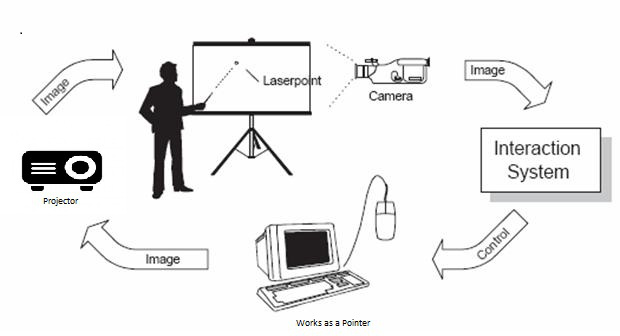
\includegraphics[width=0.48\textwidth]{abc.jpg}
	\caption{Figure 1. Laser Pointer based Interactive Projector System}
\end{wrapfigure}

Our project tries to improve the interactivity and the cost of the existing Looma system such that it can be afforded by rural schools. The use of camera to capture the projected area, and detection of location of a visual pen or other visual tools, altogether form an interactive projector system. With the use of a camera, and laser pen, our project gets scoped under \textbf{Human Computer Interaction(HCI)}. \textbf{Computer Vision(CV)} is an integral part of the interaction. The vision based HCI acts as an apt mediator between the user and the computer.

In its long term goals, our project aims to lay a foundation to improved interaction with exisiting projection systems using our hardware and software. 

\subsection{Problem Statement}
The existing wand system of Looma is basically an IR based handheld device that acts a mouse. It emits IR light, and also called a light pen. The major components of it are that it has an IR LED, a button and and on/off switch and uses 555 timer to turn the IR light source on/off. The led is blinked at a pre-determined frequency so that the blink is be analysed as a click by its camera processor. The current design uses Nintendo Wii IR camera, which is scavenged from Wii motes in order to detect the IR light on the projected screen. Some of the system's issues which can not be ignored are:

\begin{itemize}
\item \textbf {Drawing in the Whiteboard:} While drawing in the LOOMA software, the tracking of the IR led is very unreliable and the drawings are not made as expected.
\item \textbf{Use of Pre-built Multi-Object-Tracking(MOT) processor:} There is the use of inbuilt MOT processor in the camera chip, which does part of the image processing and tracking and sending coordinates. In the case of errors, its response can not be modified to remove errors which makes it inefficient
\item \textbf{Errors not detectable:} Since the Wiimote used IR to move the mouse, the location of the IR on the screen is not visible with the naked eye thus making errors not detectable 
\item \textbf{Unavailability in the market:} Wiimote IR camera chip being used in the system can not be readily bought in the open market which makes it difficult to mass produce the system
\item \textbf{Coverage and Difficult to Interact:} Wii wand is not interactive enough and works effectively only within the projected screen space which makes interacting with the screen difficult and not intuitive
\end{itemize}

In short, hacked Wii Remotes along with the Field Programmable Gate Array (FPGA) board is adding up to the cost significantly. In addition, the system is not very stable and is inefficient to use as points aforementioned, thereby leading to the research on alternative vision-based HCIs and our project is an effort to get
a prototype of one such alternative.

\subsection{Objectives}
The basic objectives of our project is make prototype for an alternative type of vision-based HCIs and in the modification of Project Looma in aspects listed below:
\begin{itemize}
	\item To use laser pointer instead of IR (Infra-red) based interaction
	\item To remove the Wii technology, and its dependencies used in current prototype thereby, making the system efficient and cost effective
\end{itemize}

\newpage
\section{LITERATURE REVIEW}
The current prototype can run off a rechargeable 12V battery, has the capability to access the World Wide Web, has readily available off line content, via established partnerships, and has an extremely easy to use interface. The device is contained in a single unit with replaceable external components (i.e. keyboard, remotes), consumes less than 100 W of power, and will cost only USD 300. The system is about the size of a shoe-box. 
As seen in the figure, the existing Looma system functional parts can be listed as:

\subsection{Looma and Wand Details}
\begin{itemize}
\item300 lumen projector
\item Internet Connected 
\item Wireless Wand control from front of room
\item Audio output for large room setting
\item Rechargeable 12V battery (8Hrs per charge)
\item Computer: Panda board
\item External ports: 1 Ethernet
\item Custom power supply (12V in 5V, 12V, 19.5V out)
\item Hacked Wii IR Camera and Wii wands
\end{itemize}

\begin{figure}[htp]
\centering
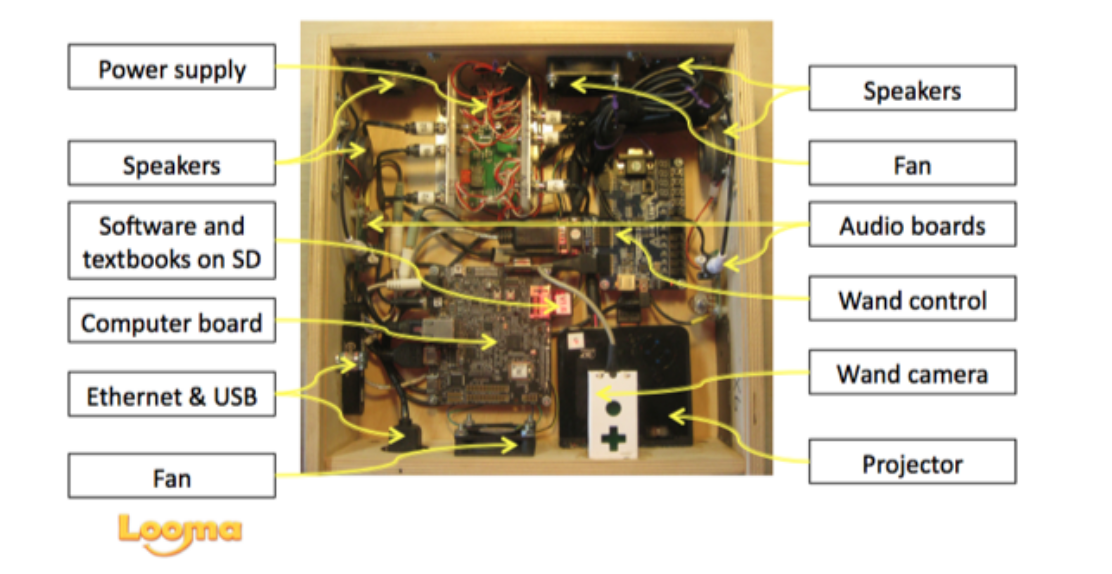
\includegraphics[scale=0.22]{looma.png}
\caption{Figure 2. Hardware and Electrical parts of Looma system}
\label{}
\end{figure}

\newpage

Wand control descriptions:
\begin{itemize}
\item Wand shown in the figure is a 3D printed IR light source
\item The wand design uses 555 timer to turn the IR light source on/off at a pre-determined frequency such that the blink can be interpreted as a click on the device
\item Current design uses Nintendo Wii IR camera, which are scavenged from Wii motes
\end{itemize}

\begin{figure}[htp]
\centering
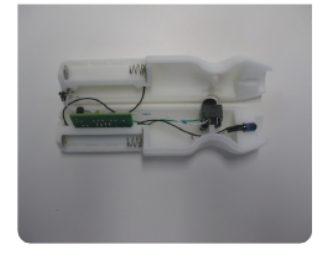
\includegraphics[scale=0.4]{wand1.png}
\caption{Figure 3. 3D printed hacked Wii Remote wand}
\label{}
\end{figure}

\subsection{System Operation Description}
\begin{figure}[htp]
\centering
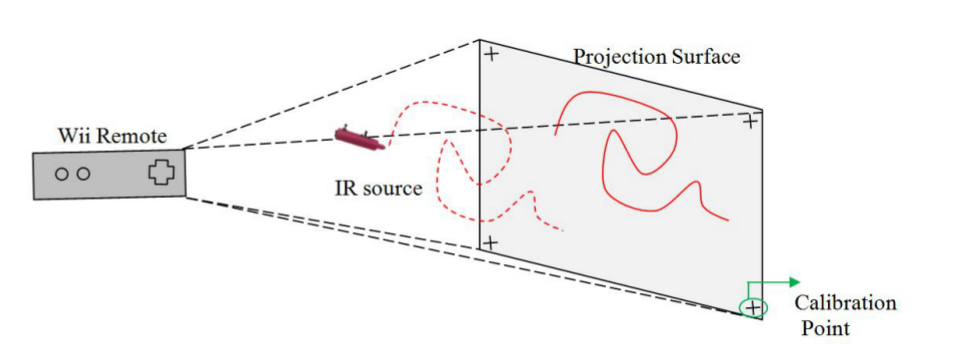
\includegraphics[scale=0.35]{wiiiii.png}
\caption{Figure 4. Illustration of how the movement of infrared is picked up by the Wiimote}
\label{}
\end{figure}

The existing system uses Wii Remote to interact in the audio-visual device. This system uses an Wii IR camera which picks up the infrared light source, and tracks it using its MOT (Multi-Object Tracking) processor present in the camera chip as shown in the figure. Wii IR Camera gives out a pre-set I2C address so the interface board needs an I2C multiplexer. To convert the I2C output to serial, and to demultiplex the signals, the system has been using an FPGA board. 

\newpage
\section{THEORITICAL BACKGROUND}
\subsection{Basic Overview}
\subsubsection{Human-computer interaction (HCI)} 
HCI is the study of how people interact with computers and to what extent computers are or are not developed for successful interaction with human beings. Developing human-computer interactions involves design on both sides of the interaction. On the technology side, the designer must have a thorough understanding of the available hardware and software components and tools. On the human side, the designer must have a good understanding of how humans learn and work with computers, including envisioning new modes of working. The designer's task is to create effective, efficient, and satisfying interactions by balancing factors such as cost, benefits, standards, and the environmental constraints in which the interaction will take place. 

Classrooms today are filled with a diverse range of students. Many of them are computer literate while others are not. Some are primarily visual learners, some are auditory learners and some kinesthetic. Others may be gifted and talented.Still others may struggle with physical, mental, behavioral or emotional challenges. In such diverse environment, it may be difficult for the teacher to cope up with each and every individual. In such cases, an effective human-computer interaction tool plays a pivotal role.Various tools are now available for the efficient human-computer interaction, one of which is the Interactive Smart Board.

The Smart Board is an interactive whiteboard that uses touch detection for user input (for example scrolling and right mouse-click) in the same way as normal PC input devices. The Smart Board interactive whiteboard operates as part of a system that includes the interactive whiteboard, a computer, a projector and whiteboarding software which can be used in various areas like offices, schools,etc.Among the various areas of application of human-computer interaction, education systems are more likely to benefit from its use.

\subsubsection{Digital Image Processing}
An image may be defined as a two-dimensional function, f(x, y), where x and y are spatial (plane) coordinates, and the amplitude of f at any pair of coordinates (x, y) is called the intensity or gray level of the image at that point. When x, y, and the amplitude values of f are all finite, discrete quantities, we call the image a digital image. The field of digital image processing refers to processing digital images by means of a digital computer.
Image processing can be defined method to convert an image into digital form and perform some operations on it, in order to get an enhanced image or to extract some useful information from it. It is a type of signal dispensation in which input is image, like video frame or photograph and output may be image or characteristics associated with that image. Usually Image Processing system includes treating images as two dimensional signals while applying already set signal processing methods to them.

The basic stages used in image processing are as follows:
\begin{enumerate}
\item Image Acquisition
\item Image Enhancement
\item Processing
\item Recognition
\end{enumerate}

\begin{enumerate}
\item \textbf{Image Acquisition}
It is the first stage of any vision system as all the other stages of image processing begin only after the acquiring of the digital image. The digital image is captured with the help of image sensor. An image sensor is a device that converts an optical image into an electronic signal such as, digital cameras, camera modules and other imaging devices. Here, Raspberry CSI camera is used for image acquisition.

\item \textbf{Image Enhancement}
After acquiring the image, the next stage is its enhancement. Image enhancement comprises the algorithms that make necessary changes to the original images so that they can be made more useful for further processing. Here, image enhancement is performed with Gaussian filter.

\item \textbf{Processing}
After the enhancement of the image, it is processed to get the further result with the respective algorithms.

\item \textbf{Recognition}
Once the  processing operations are completed, the required algorithms are applied for the feature recognition such as laser detection in our case. Here, the recognised feature is the laser pointer on the projector screen.
\end{enumerate}

\subsubsection{Embedded System}
A Microcontroller is a self-contained system with peripherals, memory and a processor that can be used as an embedded system. Most programmable microcontrollers that are used today are embedded in other consumer products or machinery including phones, peripherals, automobiles and household appliances for computer systems. Due to that, another name for a microcontroller is "embedded controller." Some embedded systems are more sophisticated, while others have minimal requirements for memory and programming length and a low software complexity. An embedded system is an engineering artifact involving computation that is subject to physical constraints(reaction constraints and execution constraints) arising through interactions of computational processes with the physical world. Reaction constraints originate from the behavioural requirements, throughput, and jitter whereas execution constraints originate from the implementation requirements and put bounds on available processor speeds, power, memory and hardware failure rates. The key to embedded systems design is to obtain desired functionality under both kinds of constraints. 

\begin{enumerate}
\item Embedded systems are application specific and single functioned
\item Efficiency is of paramount importance for embedded systems. They are optimized for energy, code size, execution time, weight and dimensions, and cost.
\item Embedded systems are typically designed to meet real time constraints; a real time system reacts to stimuli from the controlled object or operator within the time interval dictated by the environment. For real time systems, right answers arriving too late (or even too early) are wrong.
\item Embedded systems often interact (sense, manipulate and communicate) with external world through sensors and hence are typically reactive systems; a reactive system is in continual interaction with the environment and executes at a pace determined by that environment.
\item They generally have minimal or no user interface. 
\end{enumerate}

\subsection{Tools Used For Hardware}
\subsubsection{Simulation}
\paragraph {Proteus VSM}
The Proteus VSM contains mixed mode SPICE circuit simulation, animated components and microcontroller models to facilitate co-simulation of complete microcontroller based design. It is possible to develop and test such designs before a physical prototype is constructed. This is possible because interaction with the design is possible using circuit indicators like LED, display panels, actuators etc. It also provides extensive debugging facility by employing breakpoints, single stepping and variable display of both assembly code and high level language source code.

\subsubsection{Circuit Design}
\paragraph{Eagle}
Eagle is acronym for “Easily Applicable Graphical Layout” which is a flexible, expandable and scriptable schematic capture editor, PCB layout editor, auto-router and CAM and BOM tools developed by CadSoft Computer. 

\subsubsection{Microcontroller Programming}
\paragraph {AVR Studio 6}
AVR Studio 6 is a software development environment developed by Atmel. It is a full software development with an editor, simulator, programmer, etc. It comes with its own integrated C compiler, the AVR GNU C Compiler (GCC). It also supports several programmers including the STK500, AVR Dragon, etc. 

\paragraph{SinaProg}
SinaProg is Hex downloader application with AVRDude and Fuse Bit Calculator. This is used to download code/program and to set fuse bits of all AVR based microcontrollers. 

\subsection{Software implementation and simulation}
\subsubsection{Programming Language and Libraries}
\begin{enumerate}
\item Language: Python 2.7.3
IDLE is an integrated development environment for Python, which has been bundled with each release of the language. It is packaged as an optional part of the Python packaging
with many Linux distributions. It is completely written in Python and the Tkinter GUI
toolkit (wrapper functions for Tcl/Tk).According to the included README, its main
features are:
\begin{itemize}
\item Multi-window text editor with syntax highlighting, auto completion, smart indent
and other.
\item Python shell with syntax highlighting.
\item Integrated debugger with stepping, persistent breakpoints, and call stack visibility.
\end{itemize}
\item Library: OpenCV (Open Source Computer Vision Library is an open-source BSD-licensed library
that includes several hundreds of computer vision algorithms. It focuses mainly on real-
time image processing. OpenCV library has been used in python platform.
OpenCV has a modular structure, which means that the package includes several shared or
static libraries.
\begin{itemize}
\item core - a compact module defining basic data structures, including the dense
multidimensional array Mat and basic functions used by all other modules.
\item imgproc - an image processing module that includes linear and non-linear image
filtering, geometrical image transformations (resize, affine and perspective warping,
generic table-based remapping), color space conversion, histograms, and so on.
\item video - a video analysis module that includes motion estimation, background
subtraction, and object tracking algorithms.
\item calib3d - basic multiple-view geometry algorithms, single and stereo camera
calibration, and object pose estimation, stereo correspondence algorithms, and
elements of 3D reconstruction.
\item features2d - salient feature detectors, descriptors, and descriptor matchers.
\item objdetect - detection of objects and instances of the predefined classes (for
example, faces, eyes, mugs, people, cars, and so on).
\item highgui - an easy-to-use interface to video capturing, image and video codecs, as
well as simple UI capabilities.
\item gpu - GPU-accelerated algorithms from different OpenCV modules.
It also includes some other helper modules, such as FLANN and Google test wrappers,
Python bindings, and others.
\end{itemize}
\item Library: Tkinter
Standard builds of Python include an object-oriented interface to the Tcl/Tk widget set,
called \textbf{Tkinter}. This is probably the easiest to install and use. The Tkinter module (“Tk
interface”) is the standard Python interface to the Tk GUI toolkit.
Both Tk and Tkinter are available on most Unix platforms, as well as on Windows
systems. Tcl/Tk is fully portable to the MacOS, Windows, and Unix platforms.
The Tkinter module is a thin object-oriented layer on top of Tcl/Tk. Tkinter is a set of
wrappers that implement the Tk widgets as Python classes. In addition, the internal module
tkinter provides a threadsafe mechanism which allows Python and Tcl to interact.
Tkinter‘s chief virtues are that it is fast.

\item Library: Picamera
Raspberry Pi camera module can use \emph{Picamera 1.2}. It is a pure Python interace to the camera module. The interface eradicates the need to use command line syntax for grabbing image frames and videos. It does not cause restart of the camera interfaces when changing the intrinsic camera properties. 
\item Library: PyMouse
It is a pure Python cross-platform mouse control module. 

\end{enumerate}

\subsection{System Block Explanation}
\subsubsection{Projected Screen of Looma}

The Looma software runs on Looma hardware or Ubuntu. The display resolution of the screen is given by X = 1280 and Y = 768, and the display width is 60. Once the device is up, there are options of whether to use the wand or not use the wand. In the projected screen of Looma, there is a custom made user interface for the teaching materials for the students as seen in figure below.

\begin{figure}[htp]
	\centering
		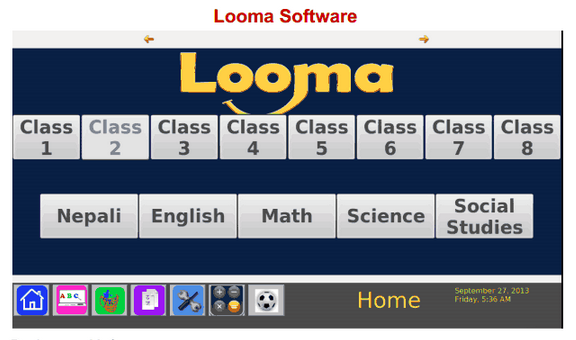
\includegraphics[scale=0.3]{loomasoftware.png}
	\caption{Figure 5. Looma Software}
\label{}
\end{figure}

\subsubsection{Raspberry Pi and Camera Board}
Raspberry Pi is a single-board computer with processor, memory, I/O ports and many more features, which together make it a functional computer for a wide range of applications in robotics. It is so simple than any logical person can program it, even it is for the first time when you work with a single-board computer.The ARM powered minicomputer is a platform with enormous possibilities and powerful enough to run many of the same programs as computer. Raspberry Pi serves as a wonderful platform for computer vision algorithms given its size, wonderful camera board and portability. Using the Picamera module, we took raw byte streams of the projected screen, and converted them to OpenCV (Open Computer Vision) object before doing further image processing algorithms.

Raspberry Pi Camera Board Module supports a full HD (High Definition) video streaming at fps of 30 with its 5 megapixel native resolution, and the sensor capable of 2592-1944 pixel static images. Raspberry Pi Camera Board Module was opted instead of normal USB web camera. 

The software of Raspberry Pi utilizes Rpi GPU (Graphical Processor Unit) when using Raspi Camera Module. So for example encoding \emph {h.264}, video has low impact on the CPU (Central Processor Unit) usage. Also, it has an excellent resolution of 5 Megapixels, which is higher than most USB webcams. It also has an excellent daytime image quality. If we use USB Webcam, it will have a very slow frame rate video and the CPU usage will be quite high. RPi does not have enough CPU horsepower to do higher frame rates, resolution and advanced video compression. 

\subsection{System Design and Description}
As seen in the figures, the images of Looma are grabbed in real time by Raspberry Pi camera board. The laser detection and click action detection algorithm is run on the Raspberry Pi.

First, the projected screen is checked for any distortion and warpness. Depending on the distortion, linear and non-linear screen coordinates mapping matrix is used. If no such distortion is present, simple linear transformation matrix is used to map the coordinates to the display resolution coordinates. The mapping matrix is saved up. The actions within the projected screen is analysed for further processing, which is our region of interest(ROI).

\begin{figure}[htp]
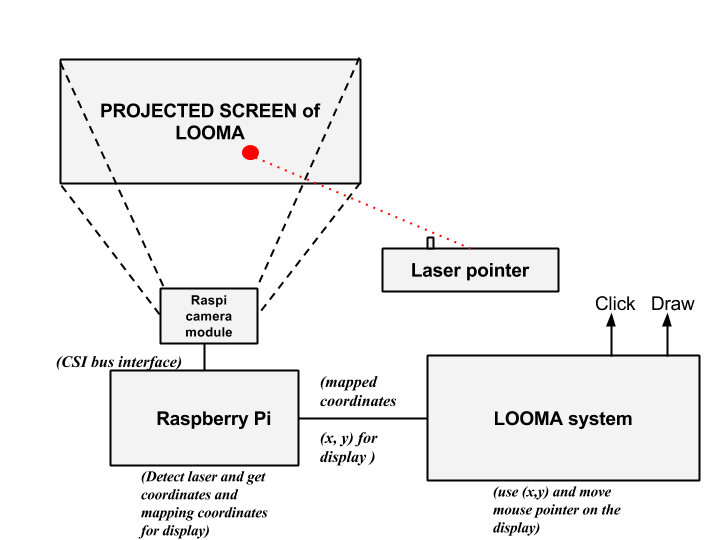
\includegraphics[scale=0.5]{proposed_system}
\caption{Figure 6. Block Diagram}
\label{Block Diagram}
\end{figure}

The next task is updating mouse as per the laser point's actions. In all conditions, whenever laser point is seen in the ROI, the mouse pointer move command is given to the system using the projector. In the case of blinks of laser point, click or drag actions is given based on the number of clicks. 

The communication between raspberry pi and the computer system is done via ethernet.

\subsection{System block and flow diagram}
\subsubsection{Block Diagram}
\begin{figure}[htp]
\centering
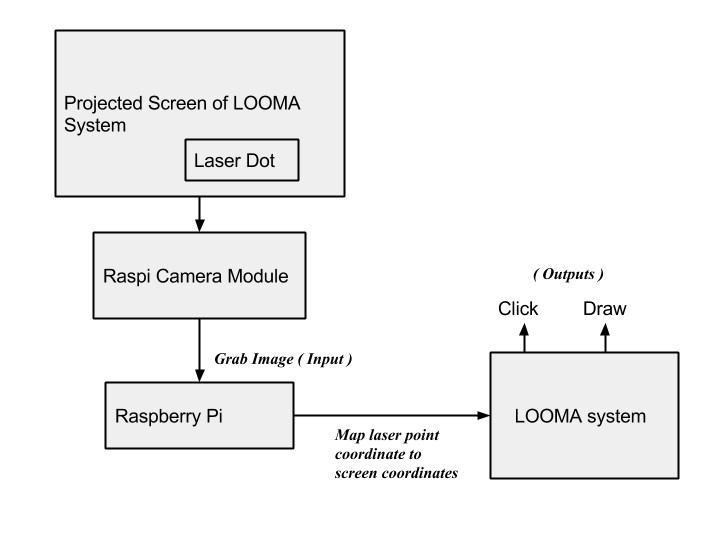
\includegraphics[scale=0.45]{block_diagram.png}
\caption{Figure 7. Block Diagram of the working of our system}
\label{ }
\end{figure}

\subsubsection{Flow Diagram}
\begin{figure}[htp]
\centering
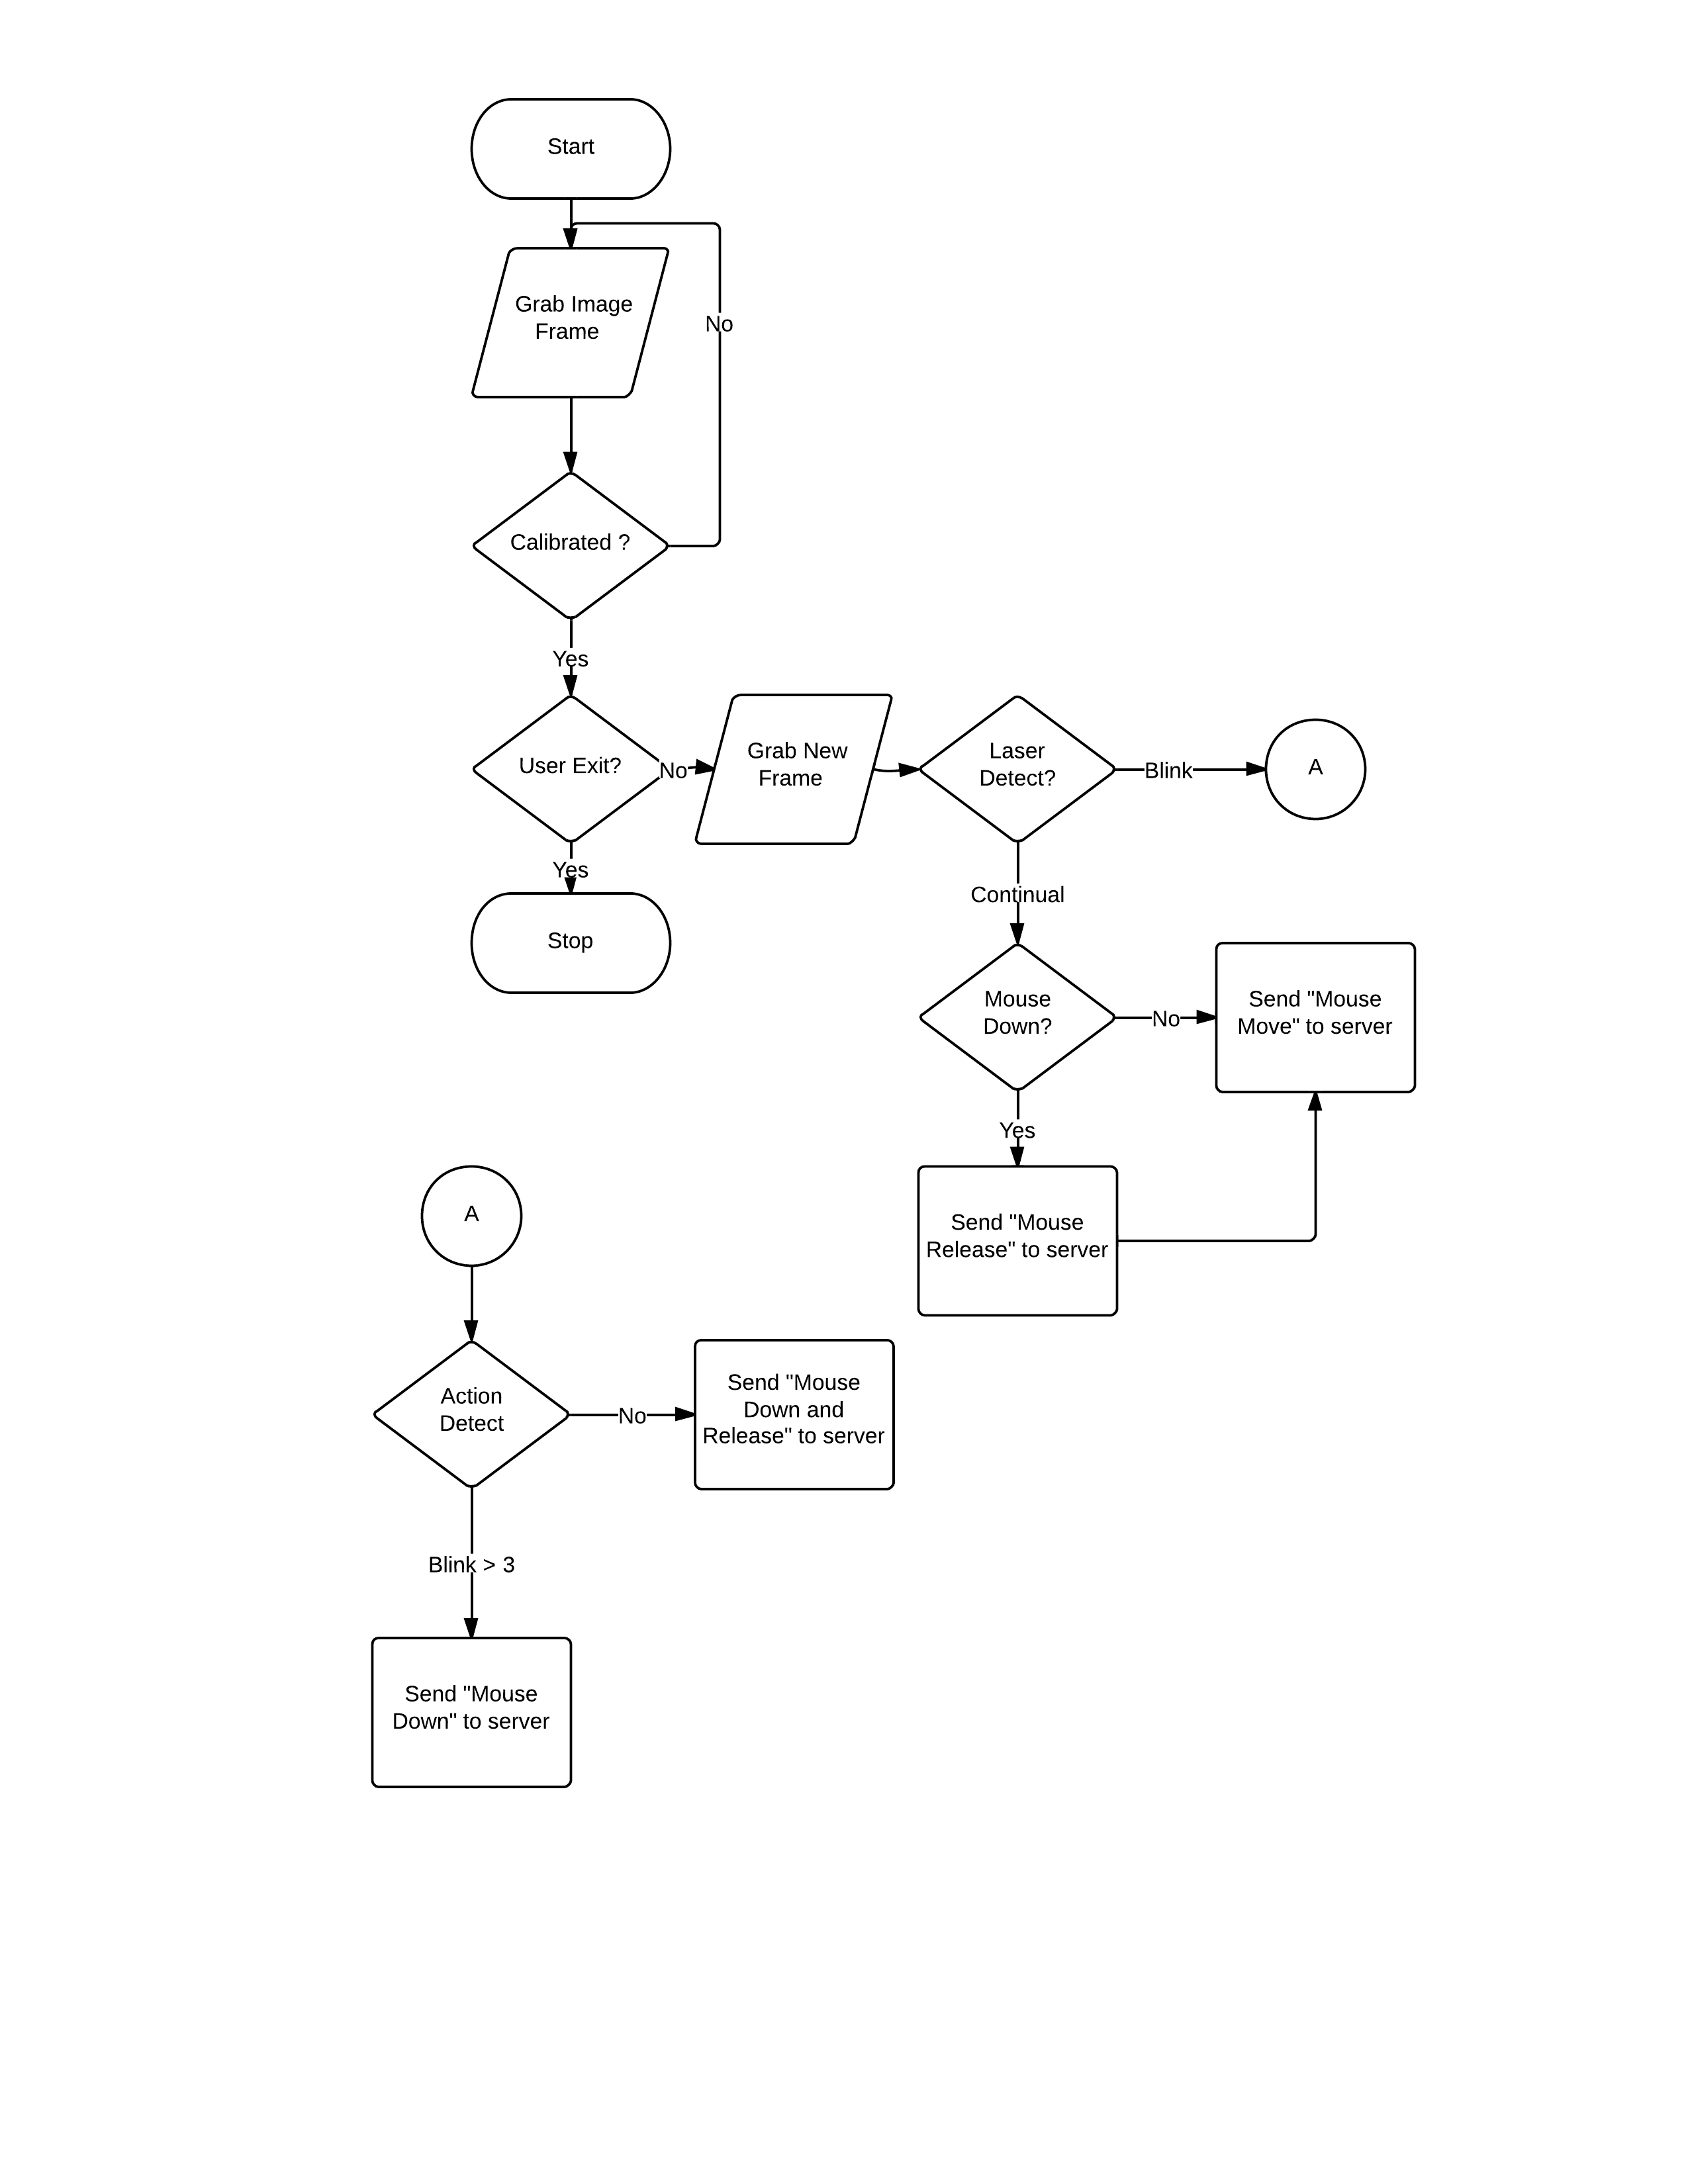
\includegraphics[scale=0.15]{flow.png}
\caption{Figure 8. Flow Diagram of our system}
\label{ }
\end{figure}

\newpage
\section{METHODOLOGY}
The main purpose of the reformed wand is to establish a way of interaction between the user and the projector system. Hence, this system needs to accomplish the following tasks to overcome the limitations provided by the current Looma wand system:
\begin{itemize}
\item Get sequence of frames from the real-time video of the projected screen
\item Use of laser light instead of infra-red for greater flexibility in the use of mouse pointer
\item Detect laser’s on or off states in each frame using image processing algorithms
\item Based on the results of detection, generate appropriate mouse press and release actions to operate mouse
\end{itemize}

\subsection{Initial Calibration of Projected Screen}
	 The projected screen is our region of interest. The four corners of the projected screen are first extracted, which is where we want our laser point to be detected within. 
	 
    The projected screen is distinguished from the wall surface by applying a threshold on the grayscale image. The applied threshold binarized the captured image such that, the grayscale image is turned into a binarized image. The projected screen is thresholded into a white surface and the rest of the image is seen as black. The contour finding algorithm is applied to this image. The contour with the largest area, which is the projected screen is obtained. The rectangular approximation of this contour gives the x and y coordinates of the projected screen. 
    
    The obtained coordinates are in the image plane coordinate system, which needs to be mapped to the projected computer’s screen coordinates. First of all, the x and y coordinates of the obtained projected screen is translated to the origin of the image plane coordinate 
The mapping is based on linear mapping technique which works on the straight undistorted projection. 

\begin{figure}[htp]
	\centering
	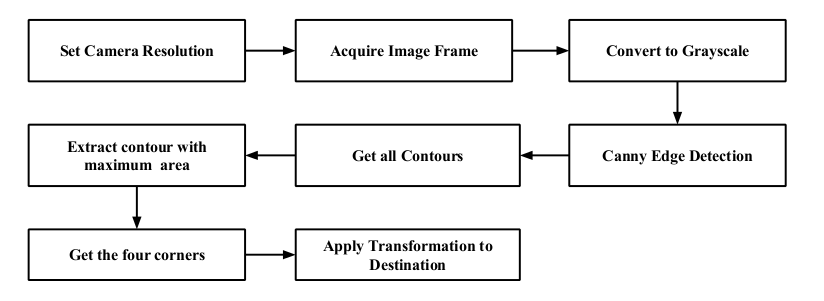
\includegraphics[scale=0.50]{Calibration.png}
	\caption{Figure 9. Calibration Process}
	\label{}
\end{figure}

\begin{enumerate}
\item Detection of edges to obtain the edge map using Canny edge algorithm
\item Detection of all contours
\item Get parent contour of contour with maximum area
\item Get the four corners of this parent contour
\item Apply the  transformation of these corners to a destination coordinates
\end{enumerate}
	
\begin{figure}[htp]
	\centering
	
\includegraphics[scale=0.20]{looma1.png}
	\caption{Figure 10. Distorted Projected Screen}
	\label{}
\end{figure}

\begin{figure}[htp]
	\centering
	
\includegraphics[scale=0.20]{result.png}
	\caption{Figure 11. Perspective Transform Correction}
	\label{}
\end{figure}

\subsection{Detection of Laser Pointer}
	Since the projected screen can comprise of all sorts of colored imagery, color based segmentation method is not appropriate for the detection of laser. For flawless detection of laser, the exposure of the camera is programmatically reduced so that laser is the only brightest pixel seen in the image frame. 
	\subsubsection{Dynamic Exposure Correction}
	A photograph's exposure determines how light or dark an image appears when it is captured by the camera. 
	
	The Raspberry Pi's camera is programmable. The camera's capture property is controlled by the camera exposure compensation parameter. The exposure correction is done as per the captured image's property dynamically. 
	
	The proper exposure configuration improves the detection of the laser. Initially, the projected screen is captured, and the camera exposure values are modified until the laser spot is the brightest in the input image. On every frame captured, the average of the value channel of the image is compared with the preset threshold and the camera exposure level is decreased accordingly if the average value of channel is greater than this threshold, the camera exposure level was decreased accordingly. 
	
\subsubsection{Brightest Pixel Detection}
After Exposure compensation is done based on the average value of the image captured, the steps involved in detecting the brighest pixel area and its location are as follow:

\textbf{Canny Edge detection:}
For the edge detection we used canny edge detection algorithm.It is a multi-stage algorithm and we will go through the following stages:
\begin{enumerate}
\item \textbf {Noise Reduction}
Since edge detection is susceptible to noise in the image, first step is to remove the noise in the image with a 5x5 Gaussian filter.

\item \textbf{Finding Intensity Gradient of the Image}
Smoothened image is then filtered with a Sobel kernel in both horizontal and vertical direction to get first derivative in horizontal direction (Gx) and vertical direction (Gy). From these two images, we can find edge gradient and direction for each pixel as follows:
\begin{figure}[htp]
\centering
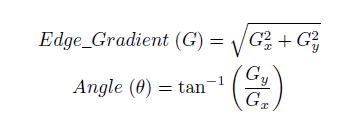
\includegraphics[scale=0.7]{canny.png}
\caption{Figure 12. Intensity Gradient and Direction}
\label{}
\end{figure}
Gradient direction is always perpendicular to edges. It is rounded to one of four angles   representing vertical, horizontal and two diagonal directions.
\item \textbf{Non maximum Suppression}
After getting gradient magnitude and direction, a full scan of image is done to remove any unwanted pixels which may not constitute the edge. For this, at every pixel, pixel is checked ­if it is a local maximum in its neighborhood in the direction of gradient.

\item \textbf{Hysteresis Thresholding}
This stage decides which are all edges are really edges and which are not. For this, we need two threshold values, minVal and maxVal. Any edges with intensity gradient more than maxVal are sure to be edges and those below minVal are sure to be non-edges, so discarded. Those who lie between these two thresholds are classified edges or non-edges based on their connectivity. If they are connected to “sure-edge” pixels, they are considered to be part of edges. Otherwise, they are also discarded.
\end{enumerate}
\begin{figure}[htp]
	\centering
	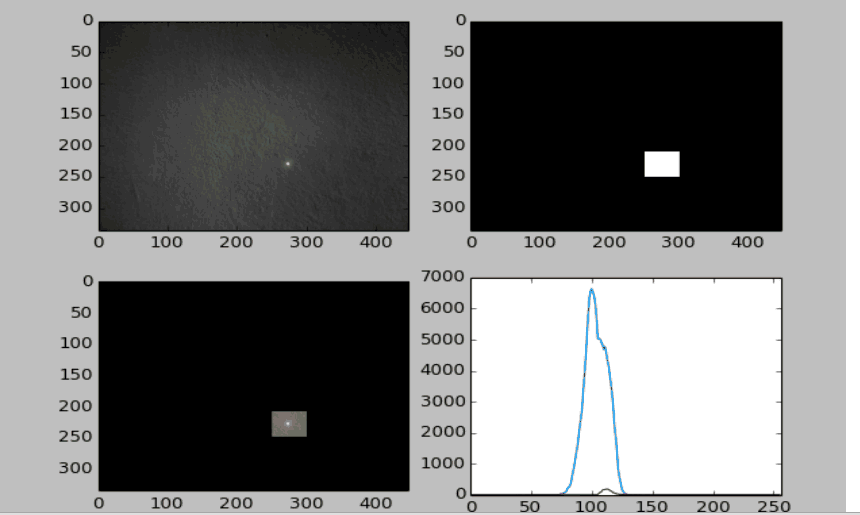
\includegraphics[scale=0.20]{histogram.png}
	\caption{Figure 13. Histogram Analysis of Brightest Pixel}
	\label{}
\end{figure}
		
\subsection{Microcontroller to generate laser pulses}

	We used an avr microcontroller instead of 555 timer so that we would not need to work with resistor values and capacitors to change the frequencies and duty cycles intermittently. Microcontroller allows us to change the values on the fly and a simple burn would allow us to change the circuit behaviour in a jiffy. Below, is the schematic of our circuit. We have implemented a circuit, that keeps laser on once power is turned on, and when the push button is pressed, it sends out a pulse at a frequency set in the microcontroller. The schematic diagram of our circuit can be followed below, and the schematic as well.
	

\begin{figure}[htp]
	\centering
	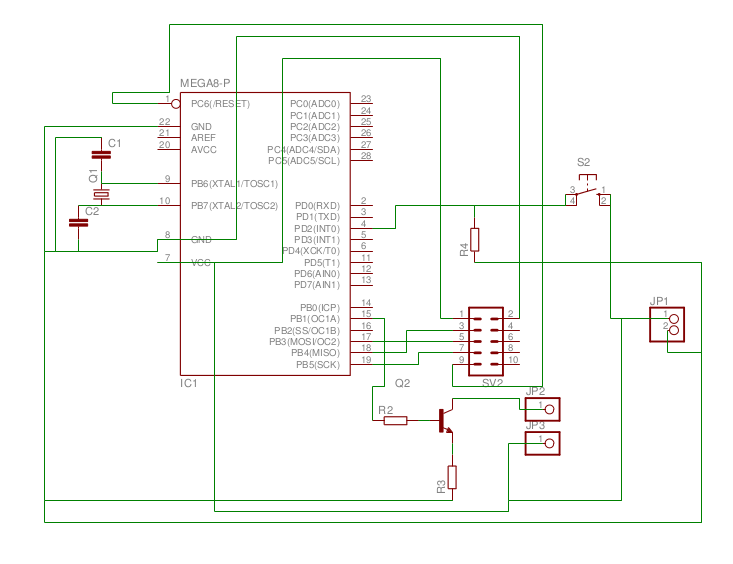
\includegraphics[scale=0.55]{schematic.png}
	\caption{Figure 14. Laser circuit schematic diagram}
	\label{}
\end{figure}

\begin{figure}[htp]
	\centering
	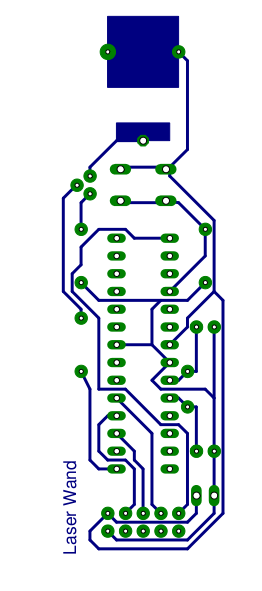
\includegraphics[scale=0.3]{eagle-non-mirror.png}
	\caption{Figure 15. Laser circuit eagle design diagram}
	\label{}
\end{figure}

	The laser circuit has been programmed such that it produces a 6Hz pulses when the push button is pressed, else it stays on. The target frequency has been set to 6Hz. The prescaler used is 64. The top value for pulse width modulation(PWM) is obtained as, 
	clock frequency/target frequency*scaler - 1. 
	 For a 20\% duty cycle, the on time of the laser is set to 20\% of the top value and off time is set to the 80\% of the top value. We have kept the push button switch in the interrupt pin, so that when the button is pushed, interrupt is obtained and the subsequent Interrupt Service Routine(ISR) can be run. This ISR does the work of producing PWM pulses of 20\% duty cycle. The diagram below is our working circuit.

\begin{figure}[htp]
	\centering
	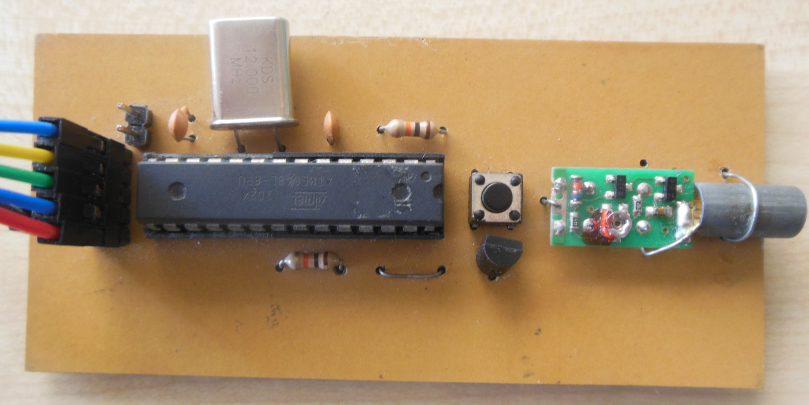
\includegraphics[scale=0.2]{front.png}
	\caption{Figure 16. Laser circuit fabricated design}
	\label{}
\end{figure}

\subsection{Hardware Implementation}
\subsubsection{Laser Wand}

A laser wand is the main interacting tool with the vision-based interactive projector system. The laser wand is a custom designed and self fabricated AVR Atmega 8L (pin diagram shown in Appendix A ) microcontroller based system. The input to the wand is a manual button press and outputs from the wand are either continual or varying laser blinks. 

On continual button press, the blinking of laser wand is made to occur at 6Hz with duty cycle of 20\%. Duty cycle is the ratio of on-time of a signal to the total time of a signal. The total time of a signal is the sum of on-time and the off-time of the signal. The on-time is the window frame of the signal, where the signal is high and off-time is the window frame of the signal, where the signal is low. So a duty cycle of 20\% implies that laser is on 20\% of the time and off 80\% of the time when the button is pressed. 

\subsubsection{Components of Laser Wand}

\subparagraph{Laser}

Laser is a device that emits light by optical amplification based on stimulated emission of electromagnetic radiation. The term \textbf{Laser} is originated as an acronym for \textbf{L}ight \textbf{A}mplification by \textbf{S}timulated \textbf{E}mission of \textbf{R}adiation. Laser light is different from other sources of light because it emits light coherently, thus allowing light to be focused on a tight spot. The laser light being used is of class IIIA, whose power output is 4mW and gives out light of wavelength 630-680nm. 

\subparagraph{Microcontroller}

The laser wand is made to blink on manual press of a button. The TIMER and PWM of the avr microcontroller is used to achieve that (configurations shown in Appendix B). 


\subsection{Finalized algorithm for click and drag}
	We constructed a State Diagram with the following states of laser.
\begin{enumerate}
\item Laser-off or 0
\item Laser-on or 1
\item Toggle 0to1 or 1to0 
\end{enumerate}

	\textbf {Laser-off} is a state of continual five or more off laser states, which occurs when the laser is not detected. \textbf{Laser-on} is a state of continual five or more on laser states, when the laser is detected. \textbf{Toggle-0to1} occurs when laser state toggles from off state to on state, whereas in \textbf{Toggle-1to0}, laser state toggles from on state to off state. 
	
	At all times, when laser is in the on state, the mouse pointer continuously moves. When laser state toggles, either from laser on to off or vice-versa, the mouse pointer is pressed. And when this mouse pointer is moving and also if the mouse pointer is in the toggled state, then the mouse starts dragging. This continues until a laser-off state or laser-on state occur, which is interpreted as a mouse release. Similarly, at every toggle state, mouse down occurs and if laser-on or laser-off state is immediately succeeded to this event, then mouse is released. This will be interpreted as click.
	
\begin{figure}[htp]
\centering
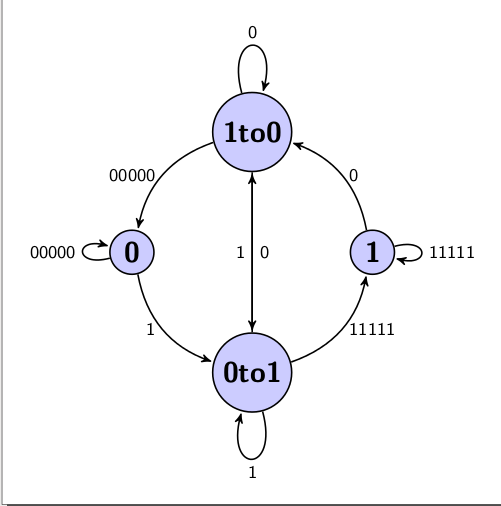
\includegraphics[scale=0.35]{state.png}
\caption{Figure 17. State Transition Diagram of Algorithm}
\label{}
\end{figure}
	
\subsection{Communication between computer and Raspberry Pi}
	A server and client program are constructed based on Transmission Control Protocol (TCP). The server and client maintain the communication between the computer and the raspberry pi. The server program is run on the computer which is being projected by the projector. The client program is run on the raspberry pi which detects laser spots. 
	
	Currently, the Looma software is obtaining the mouse coordinates through its serial port from the FPGA board. However, we implemented a protocol for communication using Transmission Control Protocol(TCP) via ethernet to communicate the mouse actions and coordinates to the computer. The Looma board was made a server, and the Raspberry Pi board a client. The client sends the coordinates of the detected laser spot, and the actions associated with it. Accordingly, the server which is listening to the client, receives the coordinates and their respective actions. The server then sends the actions to the in-built mouse application to do the desired action. 
	
\begin{figure}[htp]
\centering
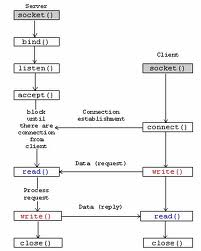
\includegraphics[scale=1]{tcp.jpeg}
\caption{Figure 18. Transmission Control Protocol}
\label{}
\end{figure}

\subsection{Movement of Mouse Pointer}
Mouse functions are provided by the PyMouse library. It runs on any Linux system running over X11 display server. It also supports Mac and Windows. PyMouse provides simple functions like move, click, press and release. PyMouse is a wrapper over Python X Library. It is used to move the mouse pointer as per the laser pointer movements. It is a fully functional X client library intended for Python programs, working as client to communicate with the X server via the X protocol. It runs on Linux using XFree86 as the server and most Unices.


The X Window System is a network-transparent window system that was designed at MIT. X display servers run on computers with either monochrome or color bitmap display hardware. Once the connection is set up, the Xlib macros are used to get the information about the current display. Similarly, using the X objects, the mouse pointer is moved by sending coordinates to the appropriate functions. 

\newpage

\section{TESTING AND RESULTS}
\subsection{Hardware Testing}

This phase of the hardware testing includes the following tests:
\begin{enumerate}
\item Connectivity testing
\item Cold solder testing
\item Checking the polarity of the capacitors
\item Testing the response of button and microcontroller
\end{enumerate}

\subsubsection{Testing the Laser Circuit}

The laser wand was tested by connecting the circuit elements as shown in the figure. Pin 1 (OC1A) and Pin 2 (OC1B) of Port B are configured in Pulse Width Modulation (PWM). Instead of laser led, a normal red-led is used. An NPN transistor is used to sink the red led to the microcontroller since it is not a good source for external circuitry. The button to control the PWM output from the Port B pins is connected to interrupt pin at Port D, pin 2.

\begin{figure}[htp]
\centering
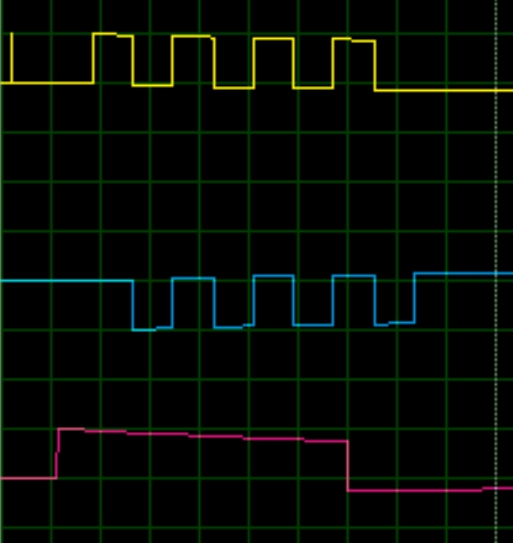
\includegraphics[scale=0.30]{afterpress.png}
\caption{Figure 19. PWM generation on button click}
\label{}
\end{figure}

Here, when button is pressed (pink line), the pwm signals are given out by pins 1 and 2 given by the other two colored lines. 

\subsection{Software Testing}
\subsubsection{Algorithm Test}

General laptop with better computing power was used at first to test the algorithm. Since the inbuilt webcam or even a USB webcam does not generally have the feature of programmatic exposure setting, a darkly lit room was used. With both server and client running in the same computer, mouse down and mouse releases were achieved with fairly high efficiency in time.

\subsubsection{System Test}

The algorithm was tested on Raspberry Pi. Raspberry Pi, the client and the Looma’s existing Pandaboard, running the server. The algorithm ran slow and was seen as inefficient due to slow processing power of raspberry pi's processing unit, hence the system ran slower.

\newpage

\section{CONCLUSION AND ENHANCEMENT}
\subsection{Conclusion}
The project \emph{Laser Pointer based Human Computer Interaction using Computer Vision} aims at providing an alternative solution to the wand system used by LOOMA. The designed system allows the user to control the projected system from a considerable distance using the laser pointer, thus aiding the teaching learning process. Though the system is designed with LOOMA in mind, it is made generic and can be used for any other system too.

   The system emphasizes on the algorithms for the detection of laser pointer on the screen and implementation of click and drag operations. By integrating the algorithm with the proper laser pointer hardware, the required laser pointer based interaction system has been developed. During the process of development, many research works and papers carried out in the respective fields were thoroughly studied. Based on the results and conclusions of these papers, the algorithms that best suited the domain of this project was selected.
   
   The system has been tested in the real working environment. Even though the system cannot process real-time data and lags in time due to the low processing power of the processor, it performs the required functions efficiently. With further enhancements, the system efficiency and speed can be increased considerably. 
   
\subsection{Problem faced and Solutions}
\subsubsection{Laser Wand}

The blinking of laser wand on manual button press by 555 timer proved to be tedious and time inefficient in case of changing frequency since it requires changing of resistors and capacitors each time. So, a microcontroller based system is designed and fabricated such that any changes in the characteristics of laser is done programmatically. 

\subsubsection{Detection of laser point by HSV Segmentation}

The laser’s distinct intensity values in the red region was utilized. However, the detection algorithm failed in cases when other points with same color and intensity. This problem is solved by considering only the brightest pixels in the projected screen. So, a exposure correction of the camera has been carried out before the start of the detection algorithm. This ensured that only laser pointer is detected.
\newpage
\subsection{COST ANALYSIS}
\subsubsection{Cost Comparison between Exisiting System and Our System}
\begin{tabular}{|c|c|c|c|c|}
\hline
	S.N  & Existing System & Cost & Designed System & Cost\\
\hline
	1 & FPGA Board and Wiring & \$117 & Raspberry Pi & \$64.90\\
\hline
	2 & Nintendo Wii Remote & \$68.89 & Raspberry Pi Camera Module & \$29.95 \\
\hline
	3 & 3D Printed IR Wands & \$20 & Laser Pointer & \$0.9\\
\hline
	4 &  &  & Atmega8L & \$1.87\\
\hline
	 & Total & \$205.89 & Total & \$97.62\\
\hline
\end{tabular}
\subsubsection{Total Cost of our Project}
\begin{tabular}{|c|c|c|c|c|}
\hline
	S.N & Items & Rate(Rs) & Quantity & Total(Rs) \\
\hline
	1 & Hydrogen Peroxide & 30 & 1 & 30 \\
\hline
	2 & Soldering Rod Bit(40W) & 250 & 1 & 250 \\
\hline
	3 & Capacitors & 10 & 2 & 20 \\
\hline
	4 & Push Button Switch & 5 & 1 & 5 \\
\hline
	5 & 12 Mhz Crystal & 35 & 1 & 35 \\
\hline
	6 & IC Base & 10 & 2 & 20 \\
\hline
	7 & Transistor & 35 & 1 & 35 \\
\hline
	8 & Drill Bit & 20 & 1 & 20 \\
\hline
	9 & PCB & 300 & 1 & 300 \\
\hline
	10 & Laser & 90 & 1 & 90 \\
\hline
	11 & Conc. HCl(250ml) & 500 & 1 & 500 \\
\hline
	12 & Aceton(250ml) & 300 & 1 & 300 \\
\hline
	13 & Atmega8L & 180 & 1 & 180 \\
\hline
	14 & Raspberry Pi & 6380.319 & 1 & 6,380.319 \\
\hline
	15 & Raspberry Pi Camera Module & 2,944.3845 & 1 & 2944.3845 \\
\hline
	16 & Laser Pointer &  0.9 & 1 & 88.479 \\
\hline 
    17 & Atmega8L & 183.8397 & 1 & 183.8397 \\
\hline
	18 & Documentation &  4000 & 1 & 4000 \\
\hline
	19 & Battery Pack & 200 & 1 & 200 \\
\hline 
    20 & Battery Holder & 50 & 1 & 50 \\
\hline 
	   & Total & & 22 & 15,443.5432\\
\hline	   
\end{tabular}	
\newline
\emph{\$1 = Rs.98.31 as of Aug 23, 2014}
\newpage
\section{Limitations and Enhancements}
\subsection{Limitations}
The limitations of the system developed in this project are as follows:
\begin{enumerate}
\item Due to the slow processing speed of the raspberry pi used, there is lag in the overall system. 
\item This system may not respond well under bright light conditions.
\item Since the raspberry pi camera is not permanently fixed to the system, a slight movement changes the calibration data of the system.
\item The slow LOOMA system processes the clicks a little later in time.
\end{enumerate}

\subsection{Enhancements}
\begin{enumerate}
\item A proper hardware with the raspberry pi system along with the camera fixed inside LOOMA can prevent the system to be calibrated each time it is moved during use.
\item A better processor than the raspberry pi can be used to enhance the system’s speed and efficiency, allowing it to perform real time operations.
\item The system performs single clicks and drag as required by the LOOMA system, but with further enhancements, it can be made to perform double clicks.
\end{enumerate}

\newpage
\section{BIBLIOGRAPHY}

\begin{enumerate}
\item Kirstein and Muller, Interaction with a Projection Screen Using a Camera-Tracked Laser Pointer,University of Dortmund, Germany
\item Mikawa, M., Morimoto, Y., Tanaka, K.: Guidance method using laser pointer and gestures for librarian robot, IEEE-RO-MAN, September, 2010
\item Johnny Chung Lee, Hacking the Nintendo Wii Remote, Carnegie Mellon University, IEEE-CS,2008 
\item Kent L. Norman, Kirk D. Norman, University of Maryland, Comparison of Relative Versus Absolute Pointing Device2, May, 2010
\item Matej MESKO, Stefan TOTH, Laser Spot Detection, University of Zilina, Faculty of Management Science and Informatics (2013) 
\item Rafael C. Gonzalez and Richard E. Woods, Digital Image Processing, 3rd Edition
\end{enumerate}

\newpage

\section{REFERENCES}
\begin{itemize}
	\item \url{www.python.org}
	\item \url{www.raspberrypi.org}
	\item \url{www.simplecv.org}
	\item \url{www.villagetechsolutions.org/}
	\item \url{www.docs.opencv.org/}
\end{itemize}
\end{document}
